\chapter{Bitcoin Transactions and Scripts}

Before Bitcoin in the late 90s there was an idea for a digital currency called \texttt{e-Cash}.
\texttt{e-Cash} introduced the concept of \textbf{blind signatures}, which allowed a bank to sign a transaction without knowing the details of the transaction.
The concept was to go a step further than plain public key cryptography, by adding a \textbf{nonce}\footnote{Random number} to be ---mathematically--- combined with the data in transit, obtaining \textit{``scrambled data''}.
The bank would \textit{``blind sign''} the scrambled data, without being able to know the original data.

\section{Bitcoin release}

Later on, in 2008, Satoshi Nakamoto\footnote{This is a pseudonym, the actual name of the author is unknown} introduced Bitcoin, a decentralized digital currency, with some key properties:
\begin{itemize}
   \item \textit{Double-spending} is prevented with a peer-to-peer network.
   \item No mint or other trusted parties.
   \item Participants can be \textit{anonymous}.
   \item New coins are made from Hashcash style \textit{proof-of-work}.
   \item The \textit{proof-of-work} for new coin generation also powers the network to prevent \textit{double-spending}
\end{itemize}

Bitcoin differs from \texttt{e-Cash} in that it is a decentralized entirely P2P system, with no central authority such as banks.

\subsection{Unhappy episodes}
In 2014 Mt GOX, a Bitcoin exchange, filed for bankruptcy after losing 850,000 Bitcoins, worth \$473 million at the time; they were most likely stolen, probably due to a vulnerability in the protocol (\textit{malleability} will be discussed later on).

Up to 2013, the Silk Road was an online black market, best known as a platform for selling illegal drugs. It was shut down by the FBI in 2013, and the founder, Ross Ulbricht, was sentenced to life in prison.

Even now, ransomware attackers demand payment in Bitcoin, as it is difficult to trace and provides pseudo anonymity through the use of Bitcoin addresses.

\section{Bitcoin Identity}
an easy way to generate new identities in a cryptographic system is to create a new random key-pair, made up of a private ---secret--- key \texttt{sk} and a public key \texttt{pk}, which acts as the ``public name'' of an user.
In case  \texttt{verify(pk, data, sig) == true} then the transaction signed with \texttt{sig} was generated by \texttt{pk}. 

\begin{figure}[htbp]
   \centering
   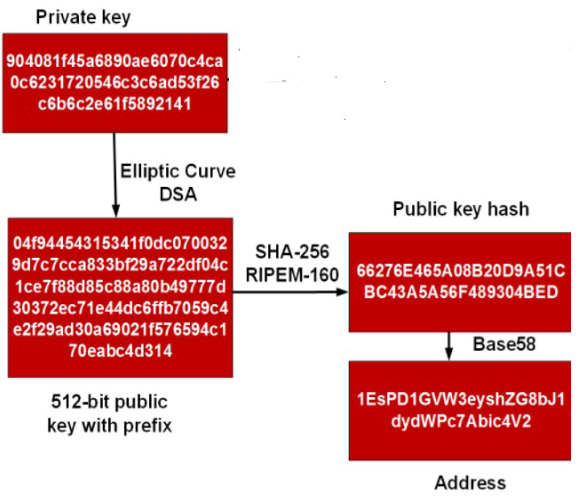
\includegraphics{images/bitcoin_addressgen.png}
   \caption{Bitcoin address generation process}
   \note{
      \texttt{Base58} is used to eliminate from the 62 alphanumerical alphabet the characters \texttt{(0,O,l,I)} which may appear identical when displayed in certain fonts.
   }
   \label{fig:bitcoin_addressgen}
\end{figure}

Addresses in the majority of cases represent the owner of a private/public key pair, and are generated using \texttt{pk}, but they may also be a \textbf{script}.

Anyone can make a new identity at any time, and such identities are not necessarily linked to any real-world identity, but the activity of an identity may be observed over time ---the blockchain is in clear readable by anyone--- and thus make inferences on who it may belong.

\section{Bitcoin Transactions}

\begin{figure}[htbp]
   \centering
   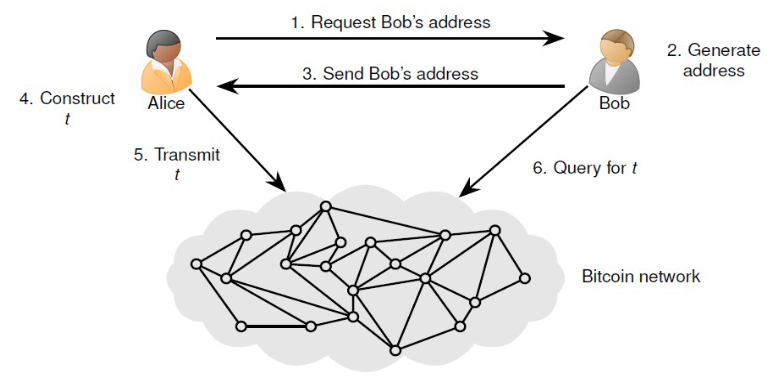
\includegraphics{images/bitcoin_workflow.png}
   \caption{Bitcoin transaction workflow}
   \note{Note that the address exchange is performed out-of-band, not through the Bitcoin P2P network}
   \label{fig:bitcoin_workflow}
\end{figure}

Is used to transfer funds from the sender to the receiver, and is registered on the blockchain when confirmed.

\begin{figure}[htbp]
   \centering
   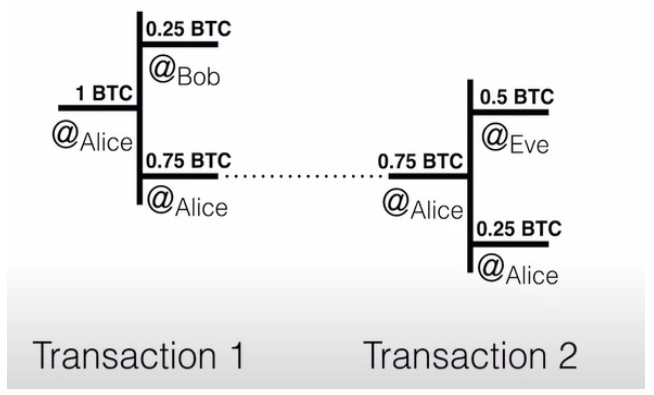
\includegraphics{images/bitcoin_transaction.png}
   \caption{Bitcoin linked transactions}
   \label{fig:bitcoin_transaction}
\end{figure}

On the left of each transaction there is a list of inputs, and on the right a list of outputs. 

In the left transaction, 0.25 is the money requested by Bob, 1.00 is the money given by Alive and 0.75 is the change she gets back.\\
Every input must equal the outputs, but note that this should include a transaction fee, computed as the difference between the inputs and the outputs, and is given to the miner who confirms the transaction.

It is possible to \textbf{merge} or \textbf{distribute}, in the first case, multiple inputs are used to create a single output, in the second case, a single input is used to create multiple outputs.\\
Transactions may also be \textbf{multi input}.

\begin{figure}[htbp]
   \centering
   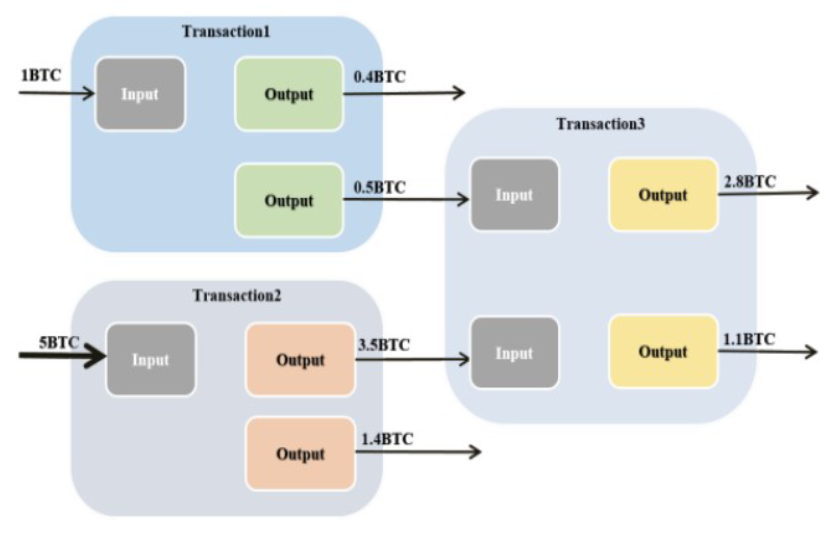
\includegraphics{images/bitcoin_multiinput.png}
   \caption{Multi input transaction}
   \label{fig:bitcoin_multiinput}
\end{figure}

\subsection{UTXO Model vs Bank Accounts}
Typical centralized currencies exploit ``bank'' accounts and \textit{transfers} between to move the money from one account (``person'') to another.
Also Ethereum follows this approach, while Bitcoin adopted the UTXO one, which is based on \textbf{unsent output addresses}, i.e. addresses containing bitcoins and not spent in any
transaction.

Each transaction input is linked (refers) the an UTXO of
a previous transaction, while each output generates a new UXTO,which is included in the user’s wallet and is available to be spent.
Each UXTO is \textit{spent} (thus is no more an UTXO) if it is linked to the input of a subsequent transaction.\\
Getting the the balance of an address, equals to scanning the network for UTXOs and adding up all the unspent output locked to that address.

\begin{figure}[htbp]
   \centering
   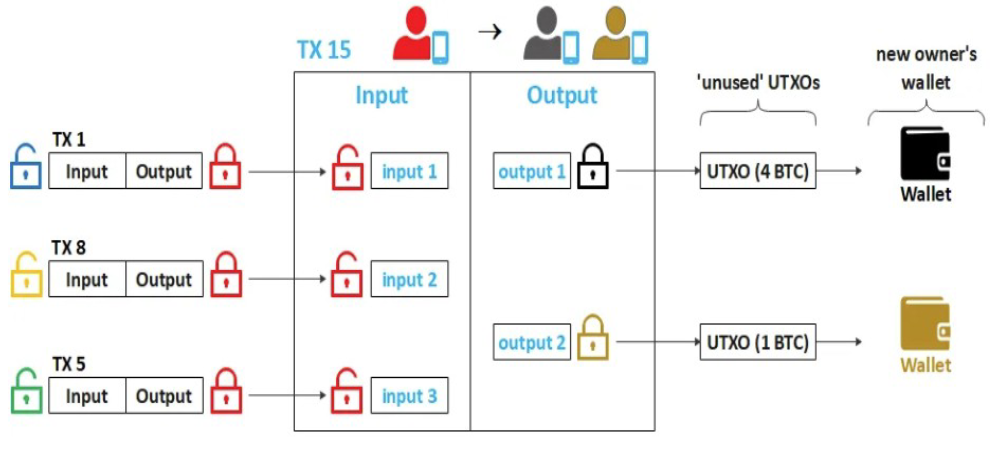
\includegraphics{images/bitcoin_UTXO.png}
   \caption{UTXO locking}

   Each UXTO \textit{``locks''} the newly generated UXTO to the new owner’s public key, and if they decide to use the UXTO in a new transaction, it must \textit{``unlock''} the funds with their private key.
   \label{fig:bitcoin_UTXO}
\end{figure}

\subsection{Scripts}
Each transaction contains a \textbf{script} written in a simple and ---intentionally--- limited language\footnote{Not Turing-complete and overall limited to avoid endless looping and execution errors.} to check the ownership of the transferred funds.\\
Script execution is stateless and completely deterministic.
Typical use case is signature verification.
Script types include:
\begin{itemize}
   \item Pay to Public Key (P2PK)
   \note{Most simple case}
   \item Pay to Public Key Hash (P2PKH)
   \note{Most common case}
   \item Pay to Script Hash (P2SH)
   \item Pay to Multi-signature
\end{itemize}

The sender appends a script on top of the sent bitcoin to lock the transferred bitcoin, and the receiver\footnote{Is it the receiver to do so?} appends a script to unlock the bitcoin.
Executing both scripts allows the receiver to spend the bitcoin.


\begin{figure}[htbp]
   \centering
   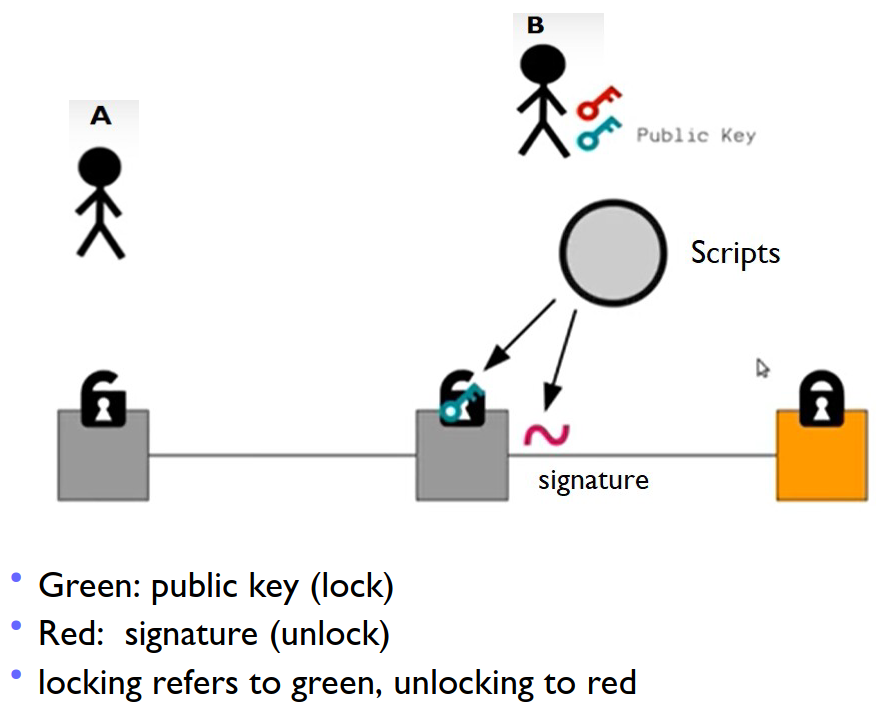
\includegraphics{images/bitcoin_script.png}
   \caption{Bitcoin script example}
   \label{fig:bitcoin_script}
\end{figure}
B first notifies its public key to A, who now knows to whom to send the bitcoin.
A unlocks some of its bitcoins ---locked by a previous transaction--- and creates a lock on the bitcoin sent to B, which can be unlocked by B using its private key.

\subsubsection*{Coinbase Transaction}
Coinbase transactions involve fresh bitcoins generated by the system used to reward miners for solving the Proof of Work, and are not linked to any previous transaction.

\subsection{Transaction Lifecycle}
\labelitemize{Lifecycle}{
   \begin{enumerate}
      \item Starts with the transaction's creation
      \item Then the transaction is signed with one or more signatures indicating the
      authorization to spend the funds referenced by the transaction.
      \item It is broadcasted on the Bitcoin P2P network
      \item Each network node (participant) validates and propagates the transaction
      until it reaches (almost) every node in the network.
      \item The transaction is verified by a mining node and included in a block of
      transactions recorded on the blockchain.
      \item Once recorded on the blockchain and confirmed by sufficient subsequent
      blocks (confirmations), the transaction is a permanent part of the blockchain
      \item The funds allocated to a new owner by the transaction can then be spent in a
      new transaction, extending the chain of ownership
   \end{enumerate}
}